% !TeX program = ptex2pdf -u -l
\documentclass[11pt,a4paper]{jsarticle}
%
\usepackage{amsmath,amssymb}
\usepackage{bm}
\usepackage[dvipdfmx]{graphicx}
\usepackage{ascmac}
\usepackage{atbegshi}
\usepackage[dvipdfmx]{geometry} % 追加: 余白を一時的に0にするため(dvipdfmx指定)
\usepackage{listings} % ソースコード表示のために追加
\usepackage{float}
\usepackage{hhline}
\usepackage{makecell} % セル内で明示改行(\\)を使うための最小変更
\usepackage{tcolorbox}
\newtcbox{\code}[1][]{
  colback=gray!10!white,
  colframe=gray!20!white,
  boxrule=0.5pt,
  left=2pt,right=2pt,top=1pt,bottom=1pt,
  box align=base,
  fontupper=\ttfamily
}
% 簡易コード表示用マクロ(本文中で\textttt{...}を使えるようにする)
\newcommand{\textttt}[1]{\texttt{#1}}
%ここからソースコードの表示に関する設定
\lstset{
  basicstyle={\ttfamily},
  identifierstyle={\small},
  commentstyle={\small\itshape},
  keywordstyle={\small\bfseries},
  ndkeywordstyle={\small},
  stringstyle={\small\ttfamily},
  frame={tb},
  breaklines=true,
  columns=[l]{fullflexible},
  numbers=left,
  xrightmargin=0zw,
  xleftmargin=3zw,
  numberstyle={\scriptsize},
  stepnumber=1,
  numbersep=1zw,
  lineskip=-0.5ex
}
\renewcommand{\lstlistingname}{ソースコード} % キャプションを「ソースコード」に変更
%ここまでソースコードの表示に関する設定
\newcommand{\myPdfAuthor}{平田爽馬/HIRATA,Soma}
\newcommand{\myPdfTitle}{EMI計測実験}
\AtBeginShipoutFirst{\special{pdf:tounicode EUC-UCS2}} % pLaTeXの内部漢字コードがEUCの場合
\AtBeginDvi{\special{pdf:docinfo <<
 /Author   (\myPdfAuthor)
 /Title    (\myPdfTitle)>>}}
%
\setlength{\textwidth}{\fullwidth}
\setlength{\textheight}{40\baselineskip}
\addtolength{\textheight}{\topskip}
\setlength{\voffset}{-0.2in}
\setlength{\topmargin}{0pt}
\setlength{\headheight}{0pt}
\setlength{\headsep}{0pt}
%
\newcommand{\divergence}{\mathrm{div}\,}  %ダイバージェンス
\newcommand{\grad}{\mathrm{grad}\,}  %グラディエント
\newcommand{\rot}{\mathrm{rot}\,}  %ローテーション
%
\title{\myPdfTitle}
\author{5E25番 平田爽馬}
\date{}
\begin{document}
%\maketitle%タイトルを挿入したくない場合は,消す
%
%
\section{目的}
私たちの周りには,妨害を発生する可能性を持つ多くの電気機器が存在している.
それらは雷に伴うサージや電磁波,人体などからの静電気放電などといった電気機器以外のものからの妨害とともに,他のものへの干渉を引き起こす可能性がある.
今回は,その中でも電気機器からの妨害の放射(EMI,日本語で電磁干渉)を計測することで,その基本を理解し,電気機器などを設計する上で必要な考えを理解する.

\section{EMCとは何か}
EMCは,Electro Magnetic Compatibilityの略であり,日本語では電磁両立性,電磁環境両立性などとも呼ばれている.
この用語は,「機器やシステムの,その環境内のいかなるものに対しても許容できない妨害を与えることなく,その電磁環境内において満足に機能する能力」のような形で定義される.
簡単に言えば,機器がその動作によってその他のものに妨害を与えず,EMCが達成されているということになる.

\subsection{なぜEMCが必要か}
EMCが欠如しているということは,何らかの干渉が発生することを意味する.
多くの人は電話やラジオへの雑音の混入やテレビの画像の乱れなどを経験したことはあるが,これもEMCが不十分であることによるものである.
やや深刻なEMC問題の身近な例の1つとしては,携帯電話とペースメーカーとの干渉の可能性が挙げられる.
私たちの周りには妨害を発生する可能性を持つ多くの電気機器が存在しており,それらは雷に伴うサージや電磁波,人体などからの静電気放電などといった電気機器以外のものからの妨害とともに,他のものへの干渉を引き起こす可能性を持っている.
このような干渉現象の例としては,表\ref{table1}に示すようなものが挙げられる.

\begin{table}[H]
\centering
\caption{干渉の例}
\label{table1}
\begin{tabular}{l|l} \hline
  \multicolumn{1}{c}{現象} & \multicolumn{1}{|c}{原因の例} \\ \hhline{=|=}
  ラジオやオーディオの雑音 & 電磁波,電源からの伝導性雑音 \\ \hline
  テレビの画像の乱れ & 電磁波,低周波磁界,電源からの伝導性雑音 \\ \hline
  テレビのゴースト & ビルからの放送波の反射 \\ \hline
  \makecell[l]{コンピュータや\\その他の電子機器の誤動作} & \makecell[l]{電磁波,電源からの伝導性雑音,\\静電気放電,サージ,電源電圧変動} \\ \hline
  照明のちらつき(フリッカ) & 電源電圧変動 \\ \hline
  \makecell[l]{変圧器の加熱,力率補償用コンデンサや\\雑音防止用コンデンサの破損} & 電源高調波電流 \\ \hline
  生体への影響 & 電磁波,低周波磁界  \\ \hline
\end{tabular}
\end{table}

\subsection{エミッションとイミュニティ}
機器からの妨害の放射(つまり,加害者としての振る舞い)は,エミッションと呼ばれる.
これは,EMI(Electro Magnetic Interface:電磁干渉)と呼ばれることもある.
また,妨害に関する耐性,すなわち妨害の受けにくさの程度はイミュニティと呼ばれる.
これは,その逆の妨害の受けやすさの程度を示す.
サセプティビリティ,あるいはEMS(Electro Magnetic Susceptibility:電磁感受性)という言葉で呼ばれることもある.
電気機器からのエミッションや電子機器への妨害の例を表\ref{table2}〜表\ref{table3}に示す.

\begin{figure}[H]
\centering
\includegraphics[width=75mm]{./fig/fig1.eps}
\caption{EMCの分類}
\label{fig1}
\end{figure}

\begin{figure}[H]
\centering
\includegraphics[width=70mm]{./fig/fig2.eps}
\caption{電子機器からの妨害の放射}
\label{fig2}
\end{figure}

\begin{table}[H]
\centering
\caption{エミッションの例}
\label{table2}
\begin{tabular}{l|l} \hline
  \multicolumn{1}{c}{発生源} & \multicolumn{1}{|c}{現象} \\ \hhline{=|=}
  \makecell[l]{放電灯,放電加工機,内燃機関の点火系,\\整流子電動機,接点の開閉,高圧線などの放電} & \makecell[l]{電磁波の放射} \\ \hline
  \makecell[l]{無線送信\\(放送,無線通信,レーダーなど)} & \makecell[l]{電磁波の意図的な放射,スプリアス} \\ \hline
  \makecell[l]{高周波エネルギー利用機器\\(高周波加熱装置,電子レンジなど)} & \makecell[l]{電磁波の放射} \\ \hline
  \makecell[l]{高周波信号利用機器\\(無線受信機,スペクトルアナライザなど)} & \makecell[l]{電磁波の放射} \\ \hline
  \makecell[l]{デジタル回路(情報技術機器,\\マイクロプロセッサ利用機器など)} & \makecell[l]{電磁波の放射,電源系統への高周波雑音や\\サージの注入,電源電圧変動の誘起(フリッカ)} \\ \hline
  \makecell[l]{交流電源(送電線,変圧器,電動機など)} & \makecell[l]{電源系統への雑音の注入,電源高調波電流} \\ \hline
\end{tabular}
\end{table}

\begin{figure}[H]
\centering
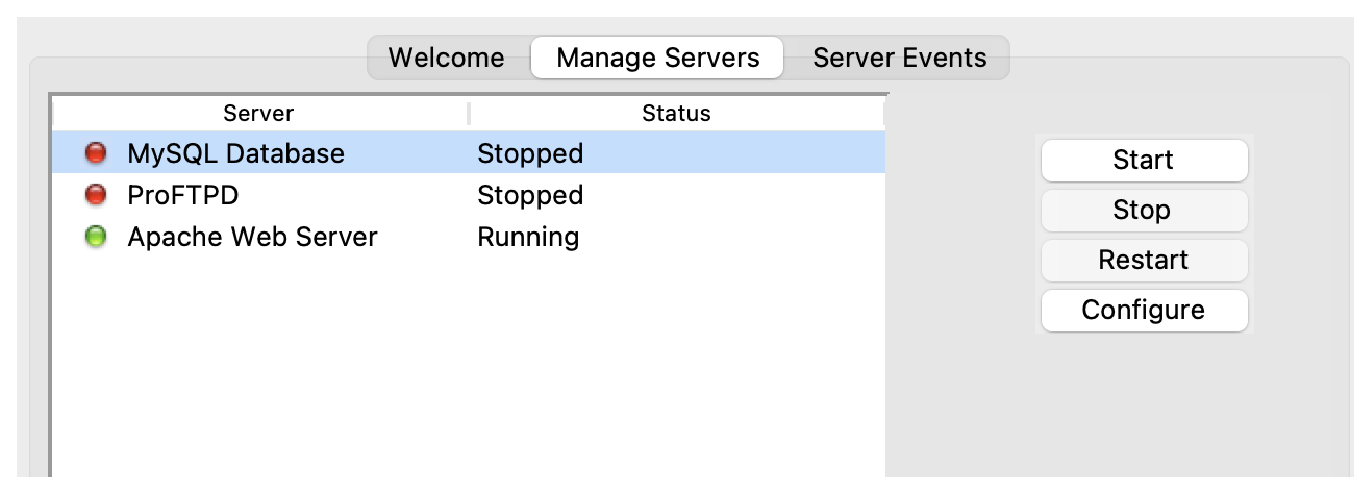
\includegraphics[width=70mm]{./fig/fig3.eps}
\caption{電子機器が外界から受ける妨害}
\label{fig3}
\end{figure}

\begin{table}[H]
\centering
\caption{イミュニティの例}
\label{table3}
\begin{tabular}{l|l} \hline
  \multicolumn{1}{c}{現象} & \multicolumn{1}{|c}{影響の例} \\ \hhline{=|=}
  \makecell[l]{電磁波} & \makecell[l]{テレビやオーディオへの雑音,\\コンピュータの誤動作,無線や有線の通信障害} \\ \hline
  \makecell[l]{電源やその他の導体を通して\\伝導する高周波ノイズ} & \makecell[l]{テレビやオーディオへの雑音,コンピュータの誤動作} \\ \hline
  \makecell[l]{静電気放電,サージ} & \makecell[l]{回路の誤動作や破壊} \\ \hline
  \makecell[l]{低周波磁界} & \makecell[l]{CRTの画像の歪み,ハム雑音} \\ \hline
  \makecell[l]{電源電圧変動や短時間の停電} & \makecell[l]{機器の機能停止や誤動作} \\ \hline
\end{tabular}
\end{table}

\subsection {EMCの達成について}
機器への干渉が問題となるのは,被害者となる危機が受ける妨害のレベルがその危機が耐えられる限界を超えた時になる(図\ref{fig4}).
従って,被害者となる危機が受ける被害のレベルを下げる(例えば,近傍にある他機器が発生する妨害を抑える)か,あるいは被害者となる機器をより強い妨害まで耐えるようにすることで,妨害のレベルその機器が耐えられる限界を超えないようにすれば,干渉が防止され,EMCが達成されたことになる.
機器の設計者がEMCを考える場合には,通常は,その機器が発生する妨害がその影響範囲内にある他のもののイミュニティ・レベルを超えないようにし,またその機器のイミュニティ・レベルをそれが受けることが予期される妨害のレベルよりも高くする必要がある.
EMCに関するさまざまな規格が作成されており,国際的な標準化(表\ref{table4},表\ref{table5}を参照)が進められている.

\begin{figure}[H]
\centering
\includegraphics[width=75mm]{./fig/fig4.eps}
\caption{イミュニティの不足による干渉の発生の概念図}
\label{fig4}
\end{figure}

\begin{table}[H]
\centering
\caption{エミッションに関する代表的な国際規格}
\label{table4}
\begin{tabular}{l|l} \hline
  \multicolumn{1}{c}{規格} & \multicolumn{1}{|c}{適用対象} \\ \hhline{=|=}
  \makecell[l]{CISPR 11} & \makecell[l]{工業,科学,及び医療(ISM)用無線周波機器} \\ \hline
  \makecell[l]{CISPR 13} & \makecell[l]{音声,及びテレビ放送受信器,及び関連機器} \\ \hline
  \makecell[l]{CISPR 14-1} & \makecell[l]{家庭用器具,電動工具,及び類似の器具} \\ \hline
  \makecell[l]{CISPR 15} & \makecell[l]{電気照明,及び類似の機器} \\ \hline
  \makecell[l]{CISPR 22} & \makecell[l]{情報技術機器} \\ \hline
  \makecell[l]{IEC 61326} & \makecell[l]{測定,制御,及び研究所での使用のための電気機器}\\ \hline
  \makecell[l]{IEC 60601-1-2} & \makecell[l]{医用電気機器,及び関連機器}\\ \hline
  \makecell[l]{IEC 61000-6-3} & \makecell[l]{住宅,商業,及び軽工業環境向けの機器(一般規格)}\\ \hline
  \makecell[l]{IEC 61000-6-4} & \makecell[l]{工業環境向けの機器(一般規格)}\\ \hline
  \makecell[l]{IEC 61000-3-2} & \makecell[l]{16A/相までの機器の高調波電流エミッション限度}\\ \hline
  \makecell[l]{IEC 61000-3-3} & \makecell[l]{16A/相までの機器の電圧変動,電圧動揺,及びフリッカの限度}\\ \hline
\end{tabular}
\end{table}

\begin{table}[H]
\centering
\caption{イミュニティに関する代表的な国際規格}
\label{table5}
\begin{tabular}{l|l} \hline
  \multicolumn{1}{c}{規格} & \multicolumn{1}{|c}{適用対象} \\ \hhline{=|=}
  \makecell[l]{CISPR 14-2} & \makecell[l]{家庭用器具,電動工具,及び類似の器具} \\ \hline
  \makecell[l]{CISPR 20} & \makecell[l]{音声,及びテレビ放送受信器,及び関連機器} \\ \hline
  \makecell[l]{CISPR 24} & \makecell[l]{情報技術機器} \\ \hline
  \makecell[l]{IEC 61326} & \makecell[l]{測定,制御,及び研究所での使用のための電気機器}\\ \hline
  \makecell[l]{IEC 60601-1-2} & \makecell[l]{医用電気機器,及び関連機器}\\ \hline
  \makecell[l]{IEC 61000-6-1} & \makecell[l]{住宅,商業,及び軽工業環境向けの機器(一般規格)}\\ \hline
  \makecell[l]{IEC 61000-6-2} & \makecell[l]{工業環境向けの機器(一般規格)}\\ \hline
\end{tabular}
\end{table}

\section{EMC規制について}
多くの地域ではEMCに関連する何らかの規制が行われており,製品を販売するためにはそれらの規制に従うことが必須となる.
他規制と同様,法的な規制はそれぞれの国や地域ごとに定められているので,規制の内容やそれに関連する手続きはその国や地域によって異なったものとなる.
これに加えて,製品の納入先によっては,その組織や産業分野に特有の規格への適合を求められることもある.
これは国家による規制のような形で法的な強制力を持つものではないが,それに従わなければその顧客(あるいはその産業分野)には製品を納入できないなど,実質的な強制力を持つものとなることもある.
この例には,軍事,航空,宇宙開発などの分野がある.
\newpage

\subsection{エミッション規制}
多くの国は,かなり昔から,主に無線障害(例えばラジオやテレビの受信障害)の防止の観点からエミッション(機器からの妨害の放射)に関する何らかの規制を行っている.
日本においては電波法があり,規定された限度値(許容される最大の放射強度)よりも強い電磁波を無許可で放射することは違法となる.
また,日本においては,一部の機器については電気用品安全法(昔の電気用品取締法)による規制も行われている.
他の国でも,同様の規制は何らかの形で行われている.
例えば,アメリカのFCC規制.EUのEMC指令は,いずれも機器からのエミッションを規制している.
規制の内容は国や地域によって,そして機器の種類によっても異なるので,機器を輸出する際には,それぞれの国や地域の該当する規定に従うことが最低条件となる.
また,国家による規制以外に,業界団体などが主導する自主規制もある.

\subsection{イミュニティ規制}
エミッションと異なり,イミュニティ(機器への妨害への耐性)が法的な規制の対象となっているケースはそれほど多くない.
この意味で,EMC指令のもとにほとんど全ての機器にイミュニティ要求が適用されるEUは例外的とも言える.
エミッションのみを規制してイミュニティを規制しないというのは,片落ちのように見えるかもしれないが,一般に,法律は機器が正しく動作することを要求してさえいないことを考えれば,これはそれほど奇妙なことでもない.
しかし,たとえイミュニティに関する法的な要求がないとしても,それはイミュニティを確保する必要がないということを意味しているわけではない.
電磁干渉に伴う問題が現実に発生しており,産業用ロボットの暴走による支障事故のような重大なものも含まれる.
特に電磁干渉によって重大な結果が引き起こされる可能性がある場合には.たとえそれが規制の対象となっていないとしても,充分なイミュニティを確保するべきである.

\section{計測システム}
図\ref{fig5}は,EMI計測システムを示す.
周囲環境から影響を受けないように電波暗室を使い,暗室内には妨害波を放射する試料(EUT)を設置する.
妨害波は,受信ATにより受信してスペクトルアナライザにより計測する.
その値は,解析ソフトにより3m法のサイトファクターの相関データ,ATやケーブル等のロス(ファクタ)を考慮して真値である妨害波のノイズ量(電界強度)を計算する.


\begin{figure}[H]
\centering
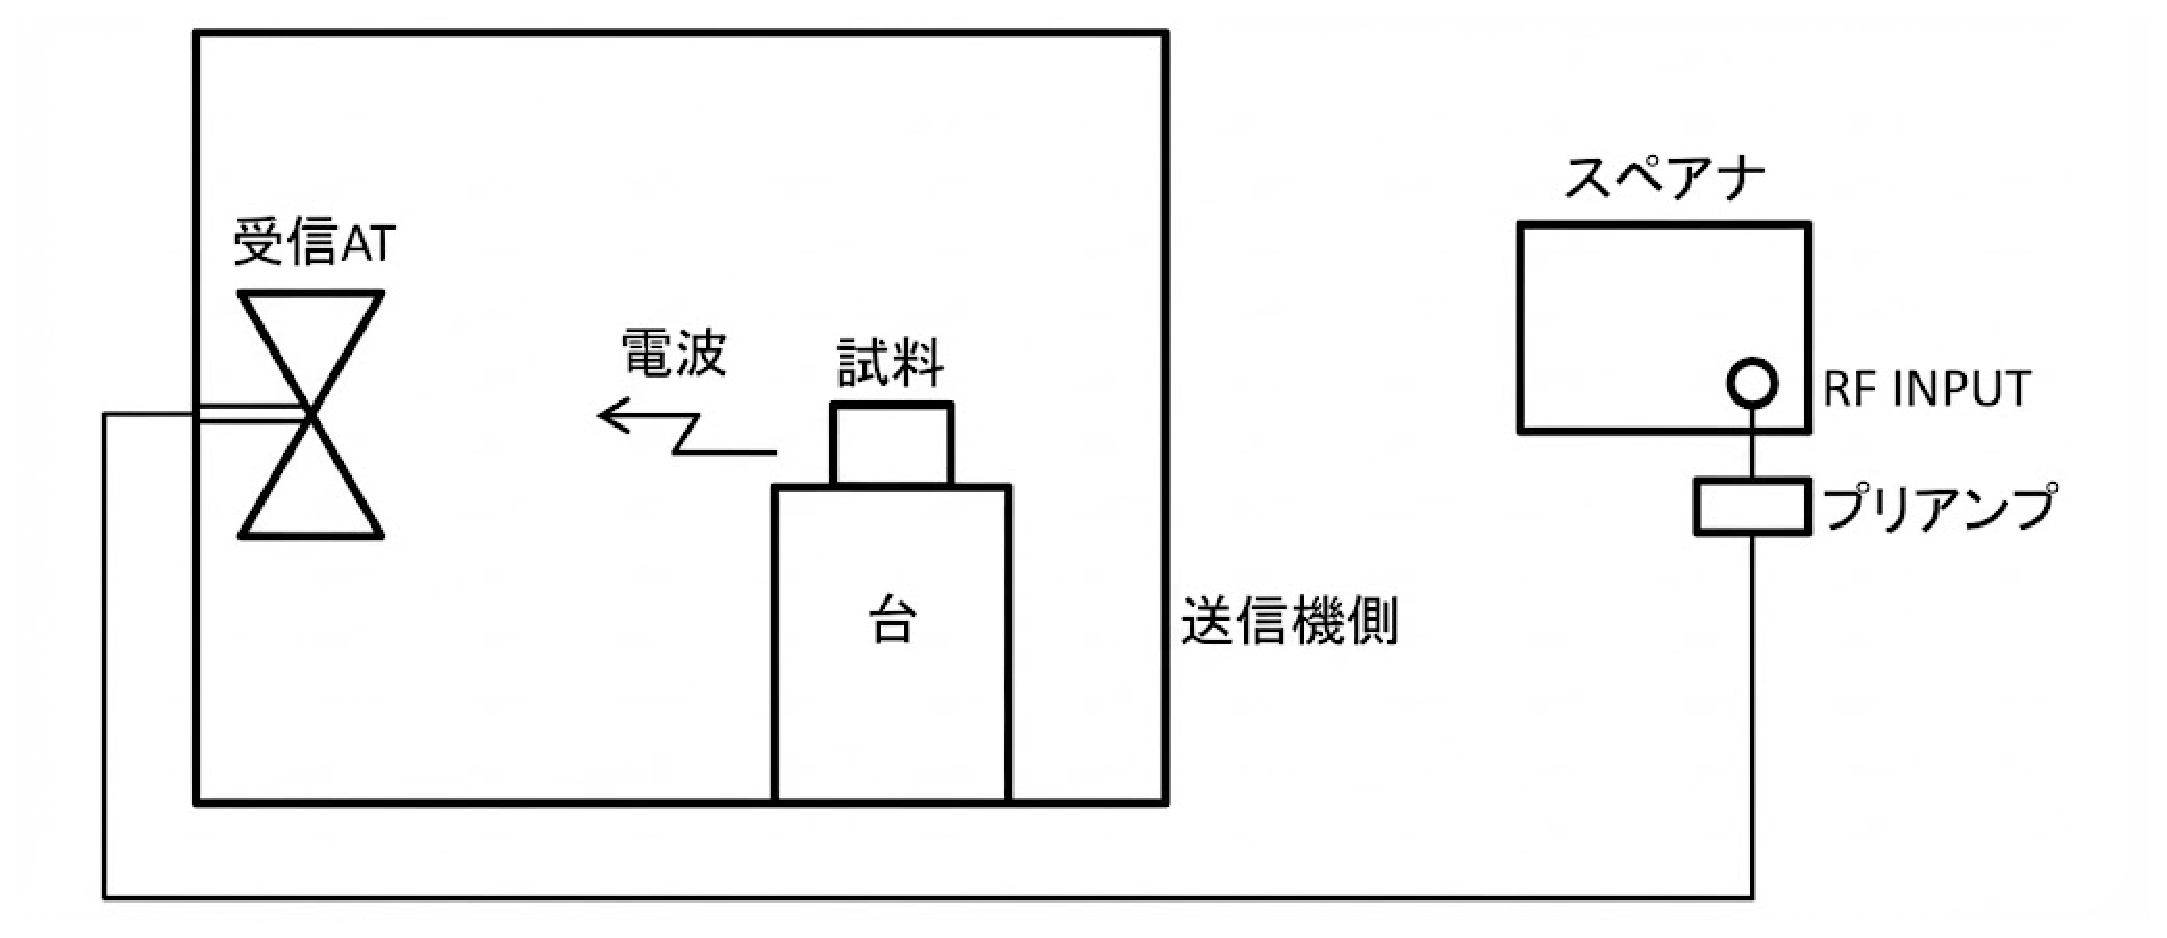
\includegraphics[width=80mm]{./fig/fig5.eps}
\caption{EMI計測システム}
\label{fig5}
\end{figure}

\begin{figure}[H]
\centering
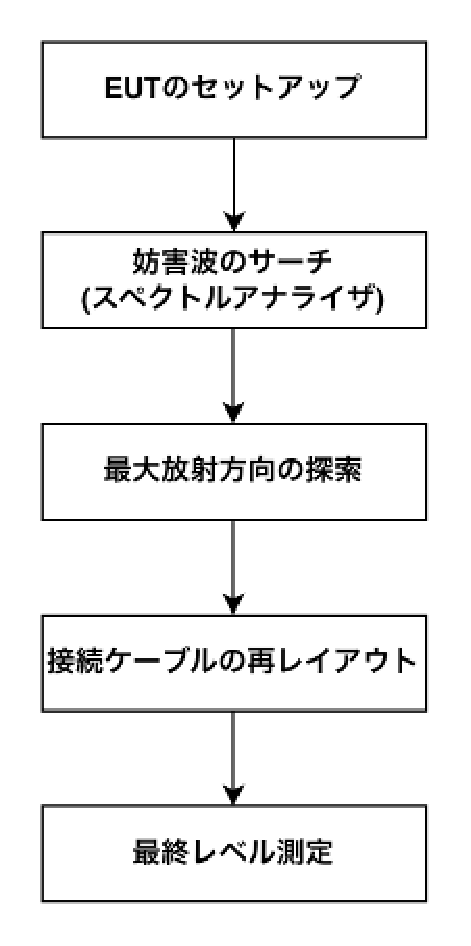
\includegraphics[width=50mm]{./fig/fig6.eps}
\caption{EMI計測の基本手順}
\label{fig6}
\end{figure}

\end{document}